\chapter{Sinterizzazione}\label{chp:Sinterizzazione}
Permette di realizzare oggetti a partire da polveri di un
materiale.

\begin{quote}
\emph{Perché sfruttare la sinterizzazione?}
\end{quote}

I motivi sono molteplici e possono essere:
\begin{itemize}
\item controllo accurato della struttura richiesta;
\item controllo della composizione chimica;
\item formabilità;
\item Quando non si vogliono macrosegregazioni;
\item realizzare dei componenti in materiali con temperatura di 
fusione particolarmente alta.
\end{itemize}

A differenza di altre lavorazioni è necessario parametrizzare la 
forma delle polveri, in quanto da quei parametri si possono ottenere 
le caratteristiche meccaniche del lavorato finale.
Inoltre la forma della polvere può essere determinante sulla
lavorazione.

Per i prodotti lavorati in sinterizzazione si parla di \eng{Net-
Shape}: ovvero, la lavorazione porta dei semilavorati già molto 
vicini alla forma finale di vendita del prodotto.
Ciò permette di usare tutto il materiale, senza avere sprechi dovuti
a delle lavorazioni che per ottenere la forma finale, devono 
eliminare parte di esso.

Data la lavorazione è possibile controllare la porosità del prodotto
come si vedrà successivamente.
In generale non si ottengono particolari caratteristiche meccaniche
anche se alle volte si possono ottenere delle caratteristiche 
migliori di altre lavorazioni già viste.

Bisogna prestare attenzione al discorso della porosità: troppa
porosità residua può essere punto di fragilità del materiale portando
alla formazione di cricche.
In più non sono facili da lavorare in post-produzione. Quindi il 
processo di produzione deve essere \eng{near net-shape} il più
possibile.

\section{La lavorazione}
Alla figura \ref{fig:ProcSint} sono riportati i principali
possibili processi per le lavorazioni di sinterizzazione.

\begin{figure}
\centering
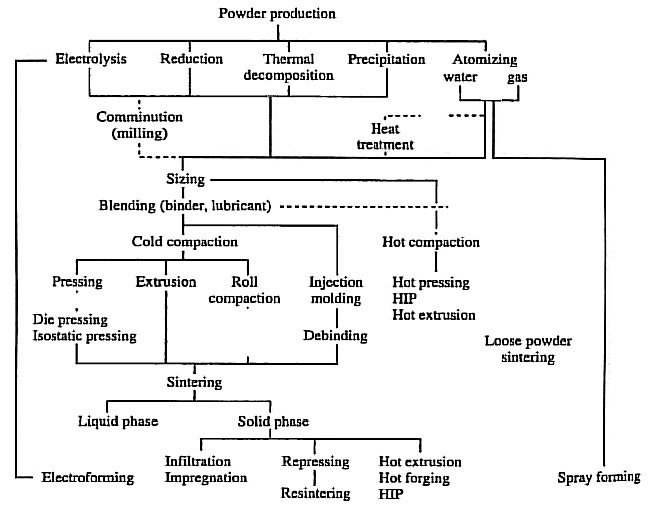
\includegraphics[width = \textwidth]{ProcSint}
\caption{Processi di produzione in sinterizzazione}
\label{fig:ProcSint}
\end{figure}

In generale il processo di sinterizzazione deve passare attraverso 
tre principali processi:

\begin{center}
\smartdiagram[sequence diagram]{Produzione Polveri, Compattazione, Sinterizzazione}
\end{center}

Sarà anche la la sequenza delle trattazioni successive.

\subsection{Produzione delle polveri}
La produzione delle polveri a partire da un semilavorato è un'operazione importate dato che, dalla caratterizzazione della polvere, si possono ottenere diverse proprietà meccaniche.
Come illustrato dalla figura \ref{fig:ProcSint}, le polveri possono essere prodotte in diverse modalità tipo:
\begin{description}
\item[Estrazione] Da un blocco di materiale si ottengono le particelle tramite:
	\begin{description}
	\item[Riduzione in ossido] dalla quale si disgrega il materiale di partenza per ossidazione e si ottiene una \textit{torta porosa}.
	\item[Decomposizione chimica] Tramite agenti chimici che attaccano il materiale di partenza si ottengono delle particelle aguzze.
	\item[Elettrolisi] Anche in questo caso si tratta di un attacco chimico e produce depositi che devono subire una successiva macinazione.
	\item[Precipitazione per soluzione acquosa] Il deposito si ha per precipitazione a partire da una soluzione liquida.
	\end{description}
\item[Deposizione] Si vaporizza il metallo per poi farlo precipitare dopo un raffreddamento. Ciò impone di prestare attenzione a quale sia la temperatura di fusione ed eventuale vaporizzazione del metallo.
\item[Atomizzazione] Può essere svolta in diverse modalità. Si sfrutta la formazione di piccole gocce di materiale fuso che, una volta raffreddate, possano diventare polvere a grana molto fine. 
In industria sono tre le modalità principalmente utilizzate, come illustrato alla figura \ref{fig:Atom}:
	\begin{enumerate}
	\item Frammentazione per fluido, in figura \ref{fig:Atom1}: dove viene fatto colare il fuso da un ugello che già forma delle gocce. Viene, poi, spruzzato del fluido, che può essere acqua o aria, per frammentare il fuso in piccole particelle. In genere si ha una relazione tipo $p_{\text{fluido}} \nearrow$ allora $D_{\text{polvere}} \searrow$.
	Bisogna comunque considerare che le particelle saranno ossidate per via del raffreddamento tramite fluido. Che può essere positivo nel caso del alluminio perché si forma allumina, non positivo per materiali ferrosi dove l'ossido forma strutture troppo dure e fragili, dannose per il prodotto post sinterizzazione.
	\item Atomizzazione centrifuga, in figura \ref{fig:Atom2}: Il colato viene spruzzato, come prima, sopra un cilindro rotante raffreddato. La forza centrifuga imposta dal cilindro alle gocce separa ulteriormente il colato formando particelle più fine. Le quali verranno raffreddate ulteriormente per il fatto che all'impatto col cilindro trovano una superficie molto più fredda.
	\item Atomizzazione con elettrodo rotante, in figura \ref{fig:Atom3}: grazie all'elettrodo si realizza un arco elettrico col materiale da polverizzare che di conseguenza si consumerà producendo la polvere. Si pone in rotazione il materiale da polverizzare. Con questo processo si ottengono delle particelle particolarmente pulite da ossidi e molto fine.
	\end{enumerate}
\item[Produzione di fibre] Non è insolito produrre delle fibre invece di polveri, le modalità sono diverse, simili a quelle viste per ottenere le polveri e sono illustrate alle figure \ref{fig:Fiber}. Le fibre hanno dei tempi di raffreddamento molto veloce: ottenendo strutture amorfe per via del fatto che il materiale non ha tempo di realizzare le strutture cristalline o non completamente.
Se si vuole ottenere fibre a partire dalla frantumazione del blocco di partenza, allora è necessario che il materiale si molto fragile.
\end{description}

Una volta ottenute le polveri e/o fibre, si passa alla caratterizzazione delle tali: ciò per mette di capire quale sia il miglior processo per la produzione.

\begin{figure}
\centering
\subfloat[][\emph{Atomizzazione per frammentazione a fluido}\label{fig:Atom1}]
{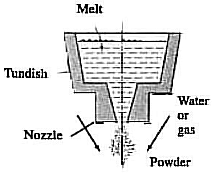
\includegraphics[width = 0.3\textwidth]{Atom1}}\:
\subfloat[][\emph{Atomizzazione tramite cilindro rotante raffreddato}%
\label{fig:Atom2}]
{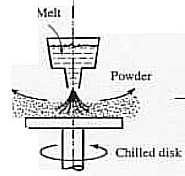
\includegraphics[width  = 0.3\textwidth]{Atom2}}\:
\subfloat[][\emph{Atomizzazione tramite elettrodo}\label{fig:Atom3}]
{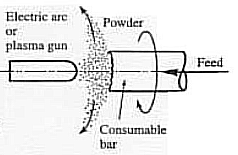
\includegraphics[width = 0.3\textwidth]{Atom3}}
\caption{Principali modalità di atomizzazione}
\label{fig:Atom}
\end{figure}

\begin{figure}
\centering
\subfloat[][\emph{Ottenimento delle fibre per frantumazione}\label{fig:Fiber1}]
{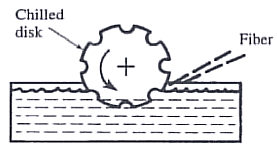
\includegraphics[width = 0.3\textwidth]{Fiber1}}\:
\subfloat[][\emph{realizzazione di fibre tramite cilindro rotante raffreddato}%
\label{fig:Fiber2}]
{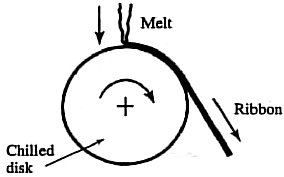
\includegraphics[width  = 0.3\textwidth]{Fiber2}}\:
\subfloat[][\emph{laminazione del fuso per ottenere delle fibre}\label{fig:Fiber3}]
{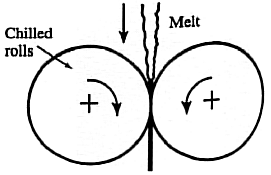
\includegraphics[width = 0.3\textwidth]{Fiber3}}
\caption{Principali modalità per ottenere delle fibre}
\label{fig:Fiber}
\end{figure}

\subsubsection{Caratterizzazione delle polveri}
Una prima caratterizzazione può essere in base alla \textbf{morfologia} della polvere.
La caratterizzazione è normata tramite ISO e si suddivide in due principlai dimensioni:
\begin{description}
\item[Forma] Le principali forme
\end{description}